
%!TEX root = ./main.tex



\tikzset{every picture/.style={line width=0.75pt}} %set default line width to 0.75pt        

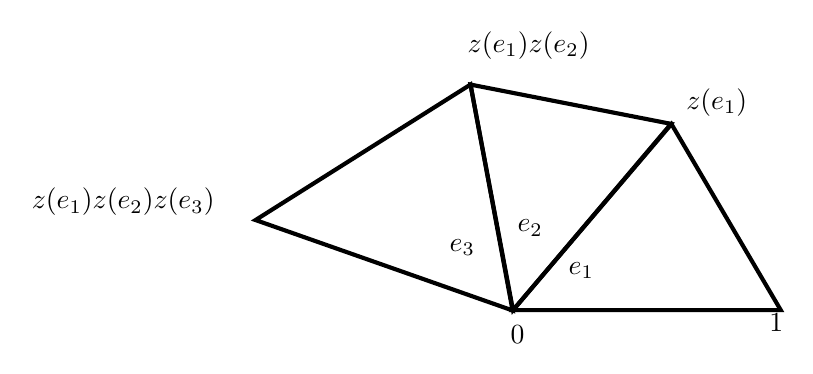
\begin{tikzpicture}[x=0.75pt,y=0.75pt,yscale=-1,xscale=1]
%uncomment if require: \path (0,300); %set diagram left start at 0, and has height of 300

%Shape: Triangle [id:dp3094193515878545] 
\draw  [line width=1.5]  (306.18,69.64) -- (402.79,88.57) -- (326.67,178.33) -- cycle ;
%Shape: Triangle [id:dp975605725949933] 
\draw  [line width=1.5]  (403,88.67) -- (455.67,178.33) -- (326.67,178.33) -- cycle ;
%Shape: Triangle [id:dp6752076580728734] 
\draw  [line width=1.5]  (326.45,178.47) -- (202.62,134.91) -- (306.18,69.64) -- cycle ;

% Text Node
\draw (352,154.07) node [anchor=north west][inner sep=0.75pt]    {$e_{1}$};
% Text Node
\draw (327.33,133.4) node [anchor=north west][inner sep=0.75pt]    {$e_{2}$};
% Text Node
\draw (294.67,142.73) node [anchor=north west][inner sep=0.75pt]    {$e_{3}$};
% Text Node
\draw (324,184.4) node [anchor=north west][inner sep=0.75pt]    {$0$};
% Text Node
\draw (448.67,178.73) node [anchor=north west][inner sep=0.75pt]    {$1$};
% Text Node
\draw (408.67,70.07) node [anchor=north west][inner sep=0.75pt]    {$z( e_{1})$};
% Text Node
\draw (303.33,42.73) node [anchor=north west][inner sep=0.75pt]    {$z( e_{1}) z( e_{2})$};
% Text Node
\draw (93.33,118.07) node [anchor=north west][inner sep=0.75pt]    {$z( e_{1}) z( e_{2}) z( e_{3})$};


\end{tikzpicture}